    %\setcounter{partie}{0} % Pour s'assurer que le compteur de \partie est à zéro dans les corrigés
    % \phantom{rrr}
    Le rectangle $ABCD$ est une réduction du rectangle $EFGH$.

    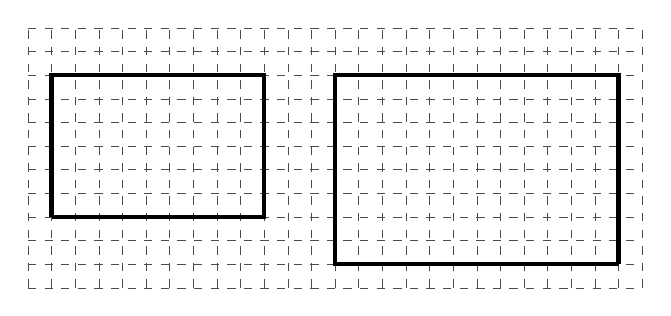
\begin{tikzpicture}[scale = 0.3]
            \draw[help lines, color=black!70, dashed] (0,0) grid (26,11);
            % points
            \coordinate (A) at (1,3);
            \coordinate (B) at (1,9);
            \coordinate (C) at (10,9);
            \coordinate (D) at (10,3);
            \coordinate (E) at (25,1);
            \coordinate (F) at (25,9);
            \coordinate (G) at (13,9);
            \coordinate (H) at (13,1);
            % rectangle ABCD
            \draw[ultra thick] (A)--(B)--(C)--(D)--(A);
            % rectangle EFGH
            \draw[ultra thick] (E)--(F)--(G)--(H)--(E);
            \tkzLabelPoints[above left](B,G);
            \tkzLabelPoints[below right](D,E);
            \tkzLabelPoints[above right](C,F);
            \tkzLabelPoints[below left](A,H);
    \end{tikzpicture}

    \begin{enumerate}
        \item Montrer que le rapport de réduction est $\dfrac{3}{4}$.

        {\color{red} $ABCD$ est une réduction de $EFGH$ donc le rapport de réduction vaut $k=\dfrac{AB}{HG}=\dfrac{6}{8}=\dfrac{3}{4}$.}
        \item Calculer l'aire des rectangles $EFGH$ puis $ABCD$.

        {\color{red}$\mathcal{A}_{EFGH}=HG\times GF=8\times 12 = 96$ unités d'aire.

        $\mathcal{A}_{ABCD}=AB\times BC=6\times 9 = 54$ unités d'aire.
        }
        \item Recopier et compléter :

        {\color{red}$\dfrac{\text{Aire de $ABCD$}}{\text{Aire de $EFGH$}}=\dfrac{54}{96}=\dfrac{9}{16}=\left(\dfrac{3}{4}\right)^2$.}
    \end{enumerate}
